% +------------------------------------------------------------------------+
% | Reference manual page: Polyhedron_3.tex
% +------------------------------------------------------------------------+
% | 17.03.1999   Lutz Kettner
% | Package: Polyhedron
% |
\RCSdef{\RCSPolyhedronRev}{$Id$}
\RCSdefDate{\RCSPolyhedronDate}{$Date$}
% +------------------------------------------------------------------------+

\ccRefPageBegin

%%RefPage: end of header, begin of main body
% +------------------------------------------------------------------------+


\begin{ccRefClass}{Polyhedron_3<Traits>}

\ccDefinition

A polyhedral surface \ccClassTemplateName\ consists of vertices $V$,
edges $E$, facets $F$ and an incidence relation on them.  Each edge is
represented by two halfedges with opposite orientations.

\begin{ccTexOnly}
    \vspace{-7mm}
    \begin{center}
      \parbox{0.4\textwidth}{%
        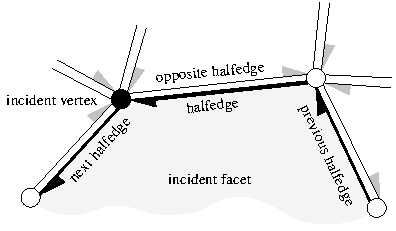
\includegraphics[width=0.4\textwidth]{Polyhedron_ref/fig/halfedge}%
      }
    \end{center}
    \vspace{-5mm}
\end{ccTexOnly}

\begin{ccHtmlOnly}
    <CENTER>
    <A HREF="fig/halfedge.gif">
        <img src="fig/halfedge_small.gif" alt="Halfedge Diagram"></A><P>
    </CENTER>
\end{ccHtmlOnly}

Vertices represent points in 3d-space. Edges are straight line segments
between two endpoints. Facets are planar polygons without holes
defined by the circular sequence of halfedges along their boundary.
The polyhedral surface itself can have holes. The halfedges
along the boundary of a hole are called {\em border halfedges\/} and
have no incident facet. An edge is a {\em border edge\/} if one of
its halfedges is a border halfedge.  A surface is {\em closed\/} if it
contains no border halfedges. A closed surface is a boundary
representation for polyhedra in three dimensions. The convention is
that the halfedges are oriented counterclockwise around facets as seen
from the outside of the polyhedron. An implication is that the
halfedges are oriented clockwise around the vertices. The notion of
the solid side of a facet as defined by the halfedge orientation
extends to polyhedral surfaces with border edges although they do not
define a closed object. If normal vectors are considered for the
facets, normals point outwards (following the right hand rule).

The strict definition can be found in~\cite{k-ugpdd-99}. One
implication of this definition is that the polyhedral surface is
always an orientable and oriented 2-manifold with border edges, i.e.,
the neighborhood of each point on the polyhedral surface is either
homeomorphic to a disc or to a half disc, except for vertices where
many holes and surfaces with boundary can join. Another implication is
that the smallest representable surface is a triangle (for polyhedral
surfaces with border edges) or a tetrahedron (for polyhedra). Boundary
representations of orientable 2-manifolds are closed under Euler
operations. They are extended with operations that create or close
holes in the surface.

Other intersections besides the incidence relation are not allowed,
although they are not automatically handled, since self intersections
are not easy to check efficiently. \ccClassTemplateName\ does only
maintain the combinatorial integrity of the polyhedral surface (using
Euler operations) and does not consider the coordinates of the points
or any geometric information.

The class \ccClassTemplateName\ can represent polyhedral surfaces as
well as polyhedra. The interface is designed in such a way that it
is easy to ignore border edges and work only with polyhedra.

The sequence of edges can be ordered in the data structure on request
such that the sequence starts with the non-border edges and ends with
the border edges. Border edges are then itself ordered such that the
halfedge which is incident to the facet comes first and the halfedge
incident to the hole comes thereafter. This normalization step counts
simultaneously the number of border edges. This number is zero if and
only if the surface is a closed polyhedron. Note that this class does
not maintain this counter nor the halfedge order during further
modifications. There is no automatic caching done for auxiliary
information.

\ccInclude{CGAL/Polyhedron_3.h}

\ccParameters

The full template declaration of \ccClassTemplateName\ states four
template parameters:

\begin{tabbing}
\ccc{template <} \=\ccc{class PolyhedronTraits_3,}\\
                 \>\ccc{class PolyhedronItems_3  = CGAL::Polyhedron_items_3,}\\
                 \>\ccc{template < class T, class I>}
                 \ccc{class HalfedgeDS = CGAL::HalfedgeDS_default,}\\
                 \>\ccc{class Alloc = CGAL_ALLOCATOR(int)>}\\
     \ccc{class Polyhedron_3;}
\end{tabbing}

The first parameter requires a model of the \ccc{PolyhedronTraits_3}
concept as argument, for example \ccc{CGAL::Polyhedron_traits_3}.  The
second parameter expects a model of the \ccc{PolyhedronItems_3}
concept.  By default, the class \ccc{CGAL::Polyhedron_items_3} is
preselected. The third parameter is a class template. A model of the
\ccc{HalfedgeDS} concept is expected. By default, the class
\ccc{CGAL::HalfedgeDS_default} is preselected, which is a list based
implementation of the halfedge data structure.
The fourth parameter \ccc{Alloc} requires a standard allocator for
\stl\ container classes. The  \ccc{rebind} mechanism from \ccc{Alloc}
will be used to create appropriate allocators internally. A default is
provided with the macro \ccc{CGAL_ALLOCATOR(int)} from the
\ccc{<CGAL/memory.h>} header file.

\ccTypes

\ccTwo{Polyhedron_3<Traits>:: circulator_category}{}

\ccNestedType{Traits}{traits class selected for \ccc{PolyhedronTraits_3}.}
\ccGlue
\ccNestedType{Items}{items class selected for \ccc{PolyhedronItems_3}.}
\ccGlue
\ccNestedType{HalfedgeDS}{instantiated halfedge data structure.}

\ccNestedType{size_type}{size type of \ccc{HalfedgeDS}.}
\ccGlue
\ccNestedType{difference_type}{difference type of \ccc{HalfedgeDS}.}
\ccGlue
\ccNestedType{iterator_category}{iterator category of \ccc{HalfedgeDS}
    for all iterators.}
\ccGlue
\ccNestedType{circulator_category}{circulator category of all circulators;
  bidirectional category if the \ccc{Items::Halfedge}  provides a \ccc{prev()}
  member function, otherwise forward category.}
\ccGlue
\ccNestedType{allocator_type}{allocator type \ccc{Alloc}.}

\ccNestedType{Vertex}{vertex type.}
\ccGlue
\ccNestedType{Halfedge}{halfedge type.}
\ccGlue
\ccNestedType{Facet}{facet type.}

\ccNestedType{Point_3}{point stored in vertices.}
\ccGlue
\ccNestedType{Plane_3}{plane equation stored in facets (if supported).}

%\ccGlue
%\ccNestedType{Normal}{normal vector stored in facets (if supported).}

The following handles, iterators, and circulators have appropriate
non-mutable counterparts, i.e., \ccc{const_handle},
\ccc{const_iterator}, and \ccc{const_circulator}. The mutable types are
assignable to their non-mutable counterparts.  Both circulators are
assignable to the \ccc{Halfedge_iterator}. The iterators are
assignable to the respective handle types. Wherever the handles appear
in function parameter lists, the corresponding iterators can be used as
well. For convenience, the \ccc{Edge_iterator} enumerates every other
halfedge. It is based on the \ccc{CGAL::N_step_adaptor} class. For
convenience, the \ccc{Point_iterator} enumerates all points in the polyhedral
surface in the same order as the \ccc{Vertex_iterator}, but with the
value type \ccc{Point}. It is based on the \ccc{CGAL::Iterator_project}
adaptor. Similarly, a \ccc{Plane_iterator} is provided.

\ccNestedType{Vertex_handle}{handle to vertex.}
\ccGlue
\ccNestedType{Halfedge_handle}{handle to halfedge.}
\ccGlue
\ccNestedType{Facet_handle}{handle to facet.}

\ccNestedType{Vertex_iterator}{iterator over all vertices.}
\ccGlue
\ccNestedType{Halfedge_iterator}{iterator over all halfedges.}
\ccGlue
\ccNestedType{Facet_iterator}{iterator over all facets.}

\ccNestedType{Halfedge_around_vertex_circulator}{circulator of
  halfedges around a vertex (cw).}
\ccGlue
\ccNestedType{Halfedge_around_facet_circulator}{circulator of
  halfedges around a facet (ccw).}

\ccNestedType{Edge_iterator}{iterator over all edges (every other halfedge).}
\ccGlue
\ccNestedType{Point_iterator}{iterator over all points.}
\ccGlue
\ccNestedType{Plane_iterator}{iterator over all plane equations.}

% +-----------------------------------+
\begin{ccAdvanced}
\ccHeading{Types for Tagging Optional Features}

\ccTwo{Polyhedron_3<Traits>:: Supports_vertex_halfedge}{}

The following types are equal to either \ccStyle{CGAL::Tag_true} or
\ccStyle{CGAL::Tag_false}, depending on whether the named feature is
supported or not.

\ccNestedType{Supports_vertex_halfedge}{\ccc{Vertex::halfedge()}.}
\ccGlue
\ccNestedType{Supports_vertex_point}{\ccc{Vertex::point()}.}
\ccGlue
\ccNestedType{Supports_halfedge_prev}{\ccc{Halfedge::prev()}.}
\ccGlue
\ccNestedType{Supports_halfedge_vertex}{\ccc{Halfedge::vertex()}.}
\ccGlue
\ccNestedType{Supports_halfedge_facet}{\ccc{Halfedge::facet()}.}
\ccGlue
\ccNestedType{Supports_facet_halfedge}{\ccc{Facet::halfedge()}.}
\ccGlue
\ccNestedType{Supports_facet_plane}{\ccc{Facet::plane()}.}
\ccGlue
\ccNestedType{Supports_removal}{supports removal of individual elements.}

%\ccGlue
%\ccNestedType{Supports_facet_normal}{\ccc{Facet::normal()}.}

\end{ccAdvanced}

\ccCreation
\ccCreationVariable{P}

\ccThree{Halfedge_iterator}{AP.m}{}
\ccThreeToTwo

\ccConstructor{Polyhedron_3(const Traits& traits = Traits());}{}

\ccConstructor{Polyhedron_3( size_type v, size_type h, size_type f,
                             const Traits& traits = Traits());}
              {a polyhedron \ccVar\ with storage reserved
               for $v$ vertices, $h$ halfedges, and $f$ facets. The
               reservation sizes are a hint for optimizing storage
               allocation.}

\ccMethod{void reserve( size_type v, size_type h, size_type f);}
              {reserve storage
               for $v$ vertices, $h$ halfedges, and $f$ facets. The
               reservation sizes are a hint for optimizing storage
               allocation. If the \ccc{capacity} is already greater
               than the requested size nothing happens. If the
               \ccc{capacity} changes all iterators and circulators
               might invalidate.}

\ccMethod{Halfedge_handle make_tetrahedron();}{a tetrahedron is added to the
    polyhedral surface. Returns a halfedge of the tetrahedron.}

\ccMethod{Halfedge_handle make_tetrahedron(const Point& p1,
                                           const Point& p2,
                                           const Point& p3,
                                           const Point& p4);}{
    a tetrahedron is added to the polyhedral surface with its
    vertices initialized to $p_1, p_2, p_3$, and $p_4$. Returns that
    halfedge of the tetrahedron which incident vertex is initialized
    to $p_1$. The incident vertex of the next halfedge is $p_2$,
    and the vertex thereafter is $p_3$.
    The remaining fourth vertex is initialized to $p_4$.}
\vspace{-3mm}

\ccMethod{Halfedge_handle make_triangle();}{a triangle with border edges is
    added to the polyhedral surface. Returns a non-border
    halfedge of the triangle.}
\vspace{-3mm}

\ccMethod{Halfedge_handle make_triangle(const Point& p1,
                                        const Point& p2,
                                        const Point& p3);}{
    a triangle with border edges is added to the polyhedral surface with its
    vertices initialized to $p_1, p_2$, and $p_3$. Returns that
    non-border halfedge of the triangle which incident vertex is initialized
    to $p_1$. The incident vertex of the next halfedge is $p_2$,
    and the vertex thereafter is $p_3$.}
\vspace{-3mm}

% +-----------------------------------+
\ccHeading{Access Member Functions}
\ccThree{Halfedge_iterator}{P.size_of_border_halfedges();}{}

\ccMethod{bool  empty() const;}{returns true if \ccVar\ is empty.}

\ccMethod{size_type size_of_vertices() const;}
    {number of vertices.}
\ccGlue
\ccMethod{size_type size_of_halfedges() const;}
    {number of halfedges (incl.\ border halfedges).}
\ccGlue
\ccMethod{size_type size_of_facets() const;}
    {number of facets.}

\ccMethod{size_type capacity_of_vertices() const;}
    {space reserved for vertices.}
\ccGlue
\ccMethod{size_type capacity_of_halfedges() const;}
    {space reserved for halfedges.}
\ccGlue
\ccMethod{size_type capacity_of_facets() const;}
    {space reserved for facets.}

\ccMethod{size_t bytes() const;}
    {bytes used for the polyhedron.}
\ccGlue
\ccMethod{size_t bytes_reserved() const;}
    {bytes reserved for the polyhedron.}

\ccMethod{allocator_type     get_allocator() const;}{allocator object.}

\ccMethod{Vertex_iterator    vertices_begin();}{iterator over all vertices.}
\ccGlue
\ccMethod{Vertex_iterator    vertices_end();}{past-the-end iterator.}
\ccGlue
\ccMethod{Halfedge_iterator  halfedges_begin();}{iterator over all
                                                 halfedges.}
\ccGlue
\ccMethod{Halfedge_iterator  halfedges_end();}{past-the-end iterator.}
\ccGlue
\ccMethod{Facet_iterator     facets_begin();}{iterator over all facets
  (excluding holes).}
\ccGlue
\ccMethod{Facet_iterator     facets_end();}{past-the-end iterator.}

\ccMethod{Edge_iterator  edges_begin();}{iterator over all edges.}
\ccGlue
\ccMethod{Edge_iterator  edges_end();}{past-the-end iterator.}

\ccMethod{Point_iterator points_begin();}{iterator over all points.}
\ccGlue
\ccMethod{Point_iterator points_end();}{past-the-end iterator.}

\ccMethod{Plane_iterator planes_begin();}{iterator over all plane equations.}
\ccGlue
\ccMethod{Plane_iterator planes_end();}{past-the-end iterator.}


\ccMethod{const Traits& traits() const;}{returns the traits class.}

% +-----------------------------------+
\ccHeading{Combinatorial Predicates}
\ccThree{Halfedge_handle}{P.split_f}{}

\ccMethod{bool is_closed() const;}{returns \ccc{true} if there are no
    border edges.}

\ccMethod{bool is_pure_bivalent() const;}{returns \ccc{true} if all
    vertices have exactly two incident edges.}

\ccMethod{bool is_pure_trivalent() const;}{returns \ccc{true} if all
    vertices have exactly three incident edges.}

\ccMethod{bool is_pure_triangle() const;}{returns \ccc{true} if all
    facets are triangles.}

\ccMethod{bool is_pure_quad() const;}{returns \ccc{true} if all
    facets are quadrilaterals.}


% +-----------------------------------+
%\ccHeading{Geometric Predicates}
%\ccThree{Halfedge_handle}{P.split_f}{}

\ccMethod{bool is_triangle( Halfedge_const_handle h) const;}{\ccc{true}
    iff the connected component denoted by $h$ is a triangle.}

\ccMethod{bool is_tetrahedron( Halfedge_const_handle h) const;}{\ccc{true}
    iff the connected component denoted by $h$ is a tetrahedron.}



% +-----------------------------------+
\ccHeading{Euler Operators (Combinatorial Modifications)}
\label{sectionPolyhedronEuler}

\ccThree{Halfedge_handle}{P.split_f}{}

The following Euler operations modify consistently the combinatorial
structure of the polyhedral surface. The geometry remains
unchanged.

\begin{ccTexOnly}
    \begin{center}
      \parbox{\textwidth}{%
          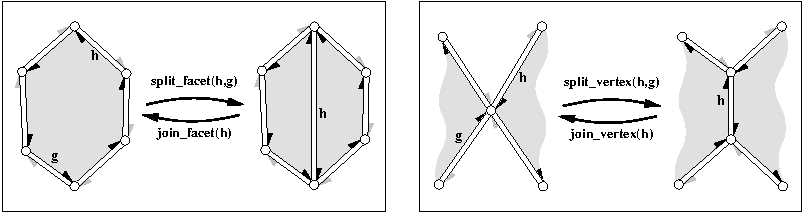
\includegraphics[width=\textwidth]{Polyhedron_ref/fig/euler}%
      }
    \end{center}
\end{ccTexOnly}

\begin{ccHtmlOnly}
    <CENTER>
    <img src="fig/euler_facet.gif" alt="Euler Operator: Facet"><P>
    </CENTER>
\end{ccHtmlOnly}


\ccMethod{Halfedge_handle split_facet( Halfedge_handle h,
                                       Halfedge_handle g);}
    {splits the facet incident to \ccc{h} and \ccc{g} into two facets
     with a new diagonal between the two vertices denoted by \ccc{h} and
     \ccc{g} respectively. The second (new) facet is a copy of the
     first facet. Returns \ccc{h->next()} after the
     operation, i.e., the new diagonal. The new face is to the right of the
     new diagonal, the old face is to the left. The time is
     proportional to the distance from \ccc{h} to \ccc{g} around the facet.
    \ccPrecond \ccc{h} and \ccc{g} are incident to the same facet.
               \ccc{h != g} (no loops). \ccc{h->next() != g} and
               \ccc{g->next() != h} (no multi-edges).}

\ccMethod{Halfedge_handle join_facet( Halfedge_handle h);}
    {joins the two facets incident to $h$. The facet incident to
      \ccc{h->opposite()} gets removed. Both facets might be
    holes. Returns the predecessor of $h$ around the facet. The invariant
    \ccc{join_facet( split_facet( h, g))} returns $h$ and keeps
    the polyhedron unchanged. The time is proportional to the size of the
    facet removed and the time to compute \ccc{h->prev()}.
    \ccPrecond The degree of both vertices incident to $h$ is at least
    three (no antennas).
    \ccCommentHeading{Requirement} \ccc{Supports_removal} $\equiv$
    \ccc{CGAL::Tag_true}.}

\begin{ccHtmlOnly}
    <CENTER>
    <img src="./fig/euler_vertex.gif" alt="Euler Operator: Vertex"><P>
    </CENTER>
\end{ccHtmlOnly}

\ccMethod{Halfedge_handle split_vertex( Halfedge_handle h,
                                        Halfedge_handle g);}
    {splits the vertex incident to \ccc{h} and \ccc{g} into two vertices,
    the old vertex remains and a new copy is created,
    and connects them with a new edge. Let \ccc{hnew} be
    \ccc{h->next()->opposite()} after the split, i.e., a halfedge
    of the new edge. The split regroups the halfedges around the two
    vertices. The halfedge sequence \ccc{hnew}, \ccc{g->next()->opposite()},
    \ldots, \ccc{h} remains around the old vertex, while the
    halfedge sequence \ccc{hnew->opposite()}, \ccc{h->next()->opposite()}
    (before the split), \ldots, \ccc{g} is regrouped around the new
    vertex. The split returns \ccc{hnew}, i.e., the new halfedge incident
    to the old vertex. The time is proportional to the distance from
    \ccc{h} to \ccc{g} around the vertex.
    \ccPrecond \ccc{h} and \ccc{g} are incident to the same vertex.
               \ccc{h != g} (antennas are not allowed).
    \ccCommentHeading{Note} A special application of the split is
    \ccc{split_vertex(h,h->next()->opposite())} which is equivalent to an
    edge split of the halfedge \ccc{h->next()} that creates a new
    vertex on the halfedge \ccc{h->next()}. See also \ccc{split_edge(h)}
    below.}

\ccMethod{Halfedge_handle join_vertex( Halfedge_handle h);}
    {joins the two vertices incident to $h$. The vertex denoted by
      \ccc{h->opposite()} gets removed. Returns the predecessor of
    $h$ around the vertex, i.e., \ccc{h->opposite()->prev()}.
    The invariant \ccc{join_vertex( split_vertex( h, g))} returns
    $h$ and keeps the polyhedron unchanged.
    The time is proportional to the degree of the vertex removed and
    the time to compute \ccc{h->prev()} and \ccc{h->opposite()->prev()}.
    \ccPrecond  The size of both facets incident to $h$ is at least
    four (no multi-edges).
    \ccCommentHeading{Requirement} \ccc{Supports_removal} $\equiv$
    \ccc{CGAL::Tag_true}.}

\ccMethod{Halfedge_handle split_edge( Halfedge_handle h);}{
    splits the halfedge \ccc{h} into two halfedges inserting a new vertex
    that is a copy of \ccc{h->opposite()->vertex()}. Is equivalent to
    \ccc{split_vertex( h->prev(), h->opposite())}. The call of \ccc{prev()}
    can make this method slower than a direct call of \ccc{split_vertex()}
    if the previous halfedge is already known and computing it would be
    costly when the halfedge data structure does not support the \ccc{prev()}
    member function. Returns the new halfedge \ccc{hnew} pointing to the
    inserted vertex. The new halfedge is followed by the old halfedge, i.e.,
    \ccc{hnew->next() == h}.}

\ccMethod{Halfedge_handle flip_edge( Halfedge_handle h);}
   {performs an edge flip. It returns $h$ after rotating the edge $h$ one
    vertex in the direction of the face orientation.
    \ccPrecond \ccc{h != Halfedge_handle()} and both  facets incident
    to $h$ are triangles.}

\begin{ccTexOnly}
    \begin{center}
      \parbox{0.52\textwidth}{%
       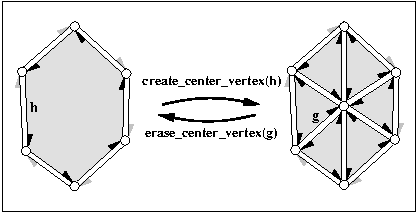
\includegraphics[width=0.52\textwidth]{Polyhedron_ref/fig/euler_center}%
      }
    \end{center}
\end{ccTexOnly}

\begin{ccHtmlOnly}
    <CENTER>
    <img src="fig/euler_center.gif" alt="Euler Operator: Center Vertex"><P>
    </CENTER>
\end{ccHtmlOnly}

\ccMethod{Halfedge_handle create_center_vertex( Halfedge_handle h);}
    {barycentric triangulation of \ccc{h->facet()}. Creates a new vertex,
     a copy of \ccc{h->vertex()}, and connects it to each vertex incident
     to \ccc{h->facet()} splitting \ccc{h->facet()} into triangles.
     \ccc{h} remains incident to the original facet, all other triangles
     are copies of this facet. Returns the halfedge \ccc{h->next()}
     after the operation, i.e., a halfedge pointing to the new vertex.
     The time is proportional to the size of the facet.
     \ccPrecond \ccc{h} is not a border halfedge.}

\ccMethod{Halfedge_handle erase_center_vertex( Halfedge_handle g);}
    {reverses \ccc{create_center_vertex}. Erases the
     vertex pointed to by \ccc{g} and all incident halfedges thereby
     merging all incident facets. Only \ccc{g->facet()} remains.
     The neighborhood of \ccc{g->vertex()} may not be triangulated,
     it can have larger facets. Returns the halfedge \ccc{g->prev()}.
     Thus, the invariant \ccc{h == erase_center_vertex(
     create_center_vertex(h))} holds if \ccc{h} is not a border halfedge.
     The time is proportional to the sum of the size of all incident facets.
     \ccPrecond None of the incident facets of \ccc{g->vertex()} is
     a hole. There are at least two distinct facets incident
     to the facets that are incident to \ccc{g->vertex()}. (This
     prevents the operation from collapsing a volume into two facets
     glued together with opposite orientations, such as would
     happen with any vertex of a tetrahedron.)
     \ccCommentHeading{Requirement}
     \ccc{Supports_removal} $\equiv$ \ccc{CGAL::Tag_true}.}


% +-----------------------------------+
\ccHeading{Euler Operators Modifying Genus}

\begin{ccTexOnly}
    \begin{center}
      \parbox{0.636\textwidth}{%
          \includegraphics[width=0.636\textwidth]%
              {Polyhedron_ref/fig/euler_loop}%
      }
    \end{center}
\end{ccTexOnly}

\begin{ccHtmlOnly}
    <CENTER>
    <img src="fig/euler_loop.gif" alt="Euler Operator: Loop"><P>
    </CENTER>
\end{ccHtmlOnly}

\ccMethod{Halfedge_handle split_loop( Halfedge_handle h,
                                      Halfedge_handle i,
                                      Halfedge_handle j);}
   {cuts the polyhedron into two parts along the cycle $(h,i,j)$ (edge \ccc{j}
    runs on the backside of the three dimensional figure above).
    Three new vertices (one copy for each vertex in the cycle) and three
    new halfedges (one copy for each halfedge in the cycle), and two new
    triangles are created. $h,i,j$ will be incident to the first new triangle.
    The return value will be the halfedge incident to the second new triangle
    which is the copy of \ccc{h-opposite()}.
    \ccPrecond $h,i,j$ denote distinct, consecutive vertices of the
    polyhedron and form a cycle: i.e., \ccc{h->vertex() ==
    i->opposite()->vertex()}, \ldots, \ccc{j->vertex() ==
    h->opposite()->vertex()}. The six facets incident to $h,i,j$ are all
    distinct.
}

\ccMethod{Halfedge_handle join_loop( Halfedge_handle h,
                                     Halfedge_handle g);}
   {glues the boundary of the two facets denoted by $h$ and $g$ together
    and returns $h$. Both facets and the vertices along the facet denoted
    by $g$ gets removed. Both facets may be holes. The invariant
    \ccc{join_loop( h, split_loop( h, i, j))} returns $h$ and keeps the
    polyhedron unchanged.
    \ccPrecond The facets denoted by $h$ and $g$ are different and have
    equal degree (i.e., number of edges).
    \ccCommentHeading{Requirement} \ccc{Supports_removal} $\equiv$
    \ccc{CGAL::Tag_true}.}

% +-----------------------------------+
\ccHeading{Modifying Facets and Holes}

\ccMethod{Halfedge_handle make_hole( Halfedge_handle h);}
    {removes the incident facet of $h$ and changes all halfedges incident
    to the facet into border edges. Returns $h$.
    See \ccc{erase_facet(h)} for a more generalized variant.
    \ccPrecond None of the incident halfedges of the facet is a border edge.
    \ccCommentHeading{Requirement} \ccc{Supports_removal} $\equiv$
    \ccc{CGAL::Tag_true}.}

\ccMethod{Halfedge_handle fill_hole( Halfedge_handle h);}{
    fills a hole with a newly created facet. Makes all border halfedges
    of the hole denoted by $h$ incident to the new facet. Returns $h$.
  \ccPrecond \ccc{h.is_border()}.}

\begin{ccTexOnly}
    \begin{center}
      \parbox{\textwidth}{%
          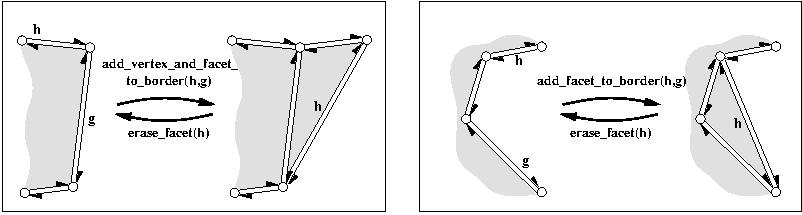
\includegraphics[width=\textwidth]{Polyhedron_ref/fig/add_facet}%
      }
    \end{center}
\end{ccTexOnly}

\begin{ccHtmlOnly}
    <CENTER>
    <img src="fig/add_facet1.gif"
     alt="Modifying Facets and Holes: add_vertex_and_facet_to_border()"><P>
    </CENTER>
\end{ccHtmlOnly}


\ccMethod{Halfedge_handle add_vertex_and_facet_to_border(
        Halfedge_handle h, Halfedge_handle g);}
   {creates a new facet within the hole incident to $h$
   and $g$ by connecting the tip of $g$ with the tip of $h$
   with two new halfedges and a new vertex and filling this separated
   part of the hole with a new facet, such that the new facet is
   incident to $g$. Returns the halfedge of the new edge that is
   incident to the new facet and the new vertex.
    \ccPrecond \ccc{h->is_border()}, \ccc{g->is_border()}, \ccc{h != g},
    and $g$ can be reached along the same hole starting with $h$.}

\begin{ccHtmlOnly}
    <CENTER>
    <img src="./fig/add_facet2.gif"
     alt="Modifying Facets and Holes: add_facet_to_border()"><P>
    </CENTER>
\end{ccHtmlOnly}

\ccMethod{Halfedge_handle add_facet_to_border( Halfedge_handle h,
                                               Halfedge_handle g);}
   {creates a new facet within the hole incident to $h$ and $g$ by
    connecting the vertex denoted by $g$ with the vertex denoted by $h$
    with a new halfedge and filling this separated part of the hole with
    a new facet, such that the new facet is incident to $g$.
    Returns the halfedge of the new edge that is incident to the new facet.
   \ccPrecond \ccc{h->is_border()}, \ccc{g->is_border()}, \ccc{h != g},
   \ccc{h->next() != g}, and $g$ can be reached along the same hole
   starting with $h$.}


% +-----------------------------------+
\ccHeading{Erasing}

\ccMethod{void erase_facet( Halfedge_handle h);}
    {removes the incident facet of $h$ and changes all halfedges incident
     to the facet into border edges or removes them from the
     polyhedral surface if they were already border edges.
     If this creates isolated vertices they get removed as well.
     See \ccc{make_hole(h)} for a more specialized variant.
     \ccPrecond \ccc{h->is_border() == false}. \ccCommentHeading{Requirement}
     \ccc{Supports_removal} $\equiv$ \ccc{CGAL::Tag_true}.}

\ccMethod{void erase_connected_component( Halfedge_handle h);}
    {removes the  vertices, halfedges, and facets that belong to the
     connected component of $h$.
     \ccCommentHeading{Requirement} \ccc{Supports_removal} $\equiv$
     \ccc{CGAL::Tag_true}.}

\ccMethod{unsigned int keep_largest_connected_components(unsigned int nb_components_to_keep);}
    {Erases the small connected components and the isolated vertices.
     Keep \ccc{nb_components_to_keep} largest connected components.
     Returns the number of connected components erased (ignoring isolated vertices).
     \ccCommentHeading{Requirement} supports vertices, halfedges, and removal operation.}

\ccMethod{void clear();}
    {removes all vertices, halfedges, and facets.}


% +-----------------------------------+
\ccHeading{Operations with Border Halfedges}

\begin{ccAdvanced}

Halfedges incident to a hole are called {\em border halfedges}. An
halfedge is a {\em border edge\/} if itself or its opposite halfedge
are border halfedges. The only requirement to work with border
halfedges is that the \ccc{Halfedge} class provides a member function
\ccc{is_border()} returning a \ccc{bool}. Usually, the halfedge data
structure supports facets and a \ccc{NULL} facet pointer will indicate
a border halfedge, but this is not the only possibility. The
\ccc{is_border()} predicate divides the edges into two classes, the
border edges and the non-border edges. The following normalization
reorganizes the sequential storage of the edges such that the
non-border edges precede the border edges, and that for each border
edge the latter one of the two halfedges is a border halfedge (the
first one is a non-border halfedge in conformance with the polyhedral
surface definition). The normalization stores the number of border
halfedges and the halfedge iterator the border edges start at within
the data structure.  Halfedge insertion or removal and changing the
border status of a halfedge invalidate these values. They are not
automatically updated.

\ccThree{Halfedge_iterator}{P.split_f}{}

\ccMethod{void   normalize_border();}
    {sorts halfedges such that the non-border edges precede the
     border edges. For each border edge the halfedge iterator will
    reference the halfedge incident to the facet right before the
    halfedge incident to the hole.}

\ccMethod{size_type size_of_border_halfedges() const;}
    {number of border halfedges.
    \ccPrecond last \ccc{normalize_border()} call still valid, see above.}

\ccMethod{size_type size_of_border_edges() const;}
    {number of border edges. Since each border edge of a polyhedral
    surface has exactly one border halfedge,
    this number is equal to \ccc{size_of_border_halfedges()}.
    \ccPrecond last \ccc{normalize_border()} call still valid, see above.}

\ccMethod{Halfedge_iterator  border_halfedges_begin();}
    {halfedge iterator starting with the border edges. The range
      [\ccStyle{halfedges_begin(), border_halfedges_begin()}) denotes
    all non-border halfedges. The range
    [\ccStyle{border_halfedges_begin(), halfedges_end()}) denotes all
    border edges.
    \ccPrecond last \ccc{normalize_border()} call still valid, see above.}

\ccMethod{Edge_iterator  border_edges_begin();}
    {edge iterator starting with the border edges. The range
      [\ccStyle{edges_begin(), border_edges_begin()}) denotes
    all non-border edges. The range
    [\ccStyle{border_edges_begin(), edges_end()}) denotes all
    border edges.
    \ccPrecond last \ccc{normalize_border()} call still valid, see above.}

\end{ccAdvanced}

% +-----------------------------------+
\ccHeading{Miscellaneous}

\ccMethod{void   inside_out();}
    {reverses facet orientations (incl.\ plane equations if supported).}

\ccMethod{bool is_valid( bool verbose = false, int level = 0) const;}
   {returns \ccc{true} if the polyhedral surface is combinatorially
    consistent. If \ccc{verbose} is \ccc{true}, statistics are
    printed to \ccc{cerr}. For \ccc{level == 1} the normalization of the
    border edges is checked too. This method checks in particular level 3 of
    \ccc{CGAL::Halfedge_data_structure_decorator::is_valid} from
    page~\ref{pageHalfedgeDSconstDecoratorRef} and that each facet is at least
    a triangle and that the two incident facets of a non-border edge are
    distinct.}

\ccMethod{bool normalized_border_is_valid( bool verbose = false) const;}{%
    returns \ccc{true} if the border halfedges are in normalized
    representation, which is when enumerating all halfedges with the
    iterator: The non-border edges precede the border edges and for
    border edges, the second halfedge is the border halfedge. The halfedge
    iterator \ccc{border_halfedges_begin()} denotes the first border
    edge. If \ccc{verbose} is \ccc{true}, statistics are
    printed to \ccc{cerr}.
}

\newpage
\begin{ccAdvanced}
\ccMethod{void  delegate( CGAL::Modifier_base<HDS>& m);}
    {calls the \ccc{operator()} of the modifier $m$. See
    \ccc{CGAL::Modifier_base} for a
    description of modifier design and its usage.
    \ccPrecond The polyhedral surface must be valid when the modifier
    returns from execution.}
\end{ccAdvanced}

\ccSeeAlso

\ccRefIdfierPage{CGAL::Polyhedron_3<Traits>::Vertex}\\
\ccRefIdfierPage{CGAL::Polyhedron_3<Traits>::Halfedge}\\
\ccRefIdfierPage{CGAL::Polyhedron_3<Traits>::Facet}\\
\ccRefConceptPage{PolyhedronTraits_3}\\
\ccRefIdfierPage{CGAL::Polyhedron_traits_3<Kernel>}\\
\ccRefConceptPage{PolyhedronItems_3}\\
\ccRefIdfierPage{CGAL::Polyhedron_items_3}\\
\ccRefConceptPage{HalfedgeDS}\\
\ccRefIdfierPage{CGAL::HalfedgeDS_default}\\
\ccRefIdfierPage{CGAL::Polyhedron_incremental_builder_3<HDS>}\\
\ccc{CGAL::Modifier_base}.

\ccExample


This example program instantiates a polyhedron using the default
traits class and creates a tetrahedron.

\ccIncludeExampleCode{Polyhedron/polyhedron_prog_simple.cpp}

\end{ccRefClass}

% +------------------------------------------------------------------------+
%%RefPage: end of main body, begin of footer
\ccRefPageEnd
% EOF
% +------------------------------------------------------------------------+

